\documentclass[11pt,TP,2A]{tdtp}
\usepackage[utf8]{inputenc}
\usepackage[french]{babel}
\usepackage{listings} 
\usepackage{graphicx}
\usepackage{subfigure}
\usepackage{listings}
\usepackage{minted}

\tcbuselibrary{minted,breakable}

\usepackage{booktabs}
\usepackage{xcolor}
\usepackage{listings}

\lstset{
  showspaces=false,
  showstringspaces=false,
  breaklines=true,
  columns=fixed,
  extendedchars=true,
  stringstyle=\sf,
  identifierstyle=\sf,
  ndkeywordstyle=\sf,
  mathescape=false,
  basicstyle=\footnotesize, 
  frame=single,
  rulesepcolor=\color{black}, 
}

% Style code
\lstdefinestyle{code}
{
frame=shadowbox, 
numbers=right,
columns=fullflexible,
rulesepcolor=\color{black}, % Fond noir du shadowbox
%xleftmargin=0.5cm, xrightmargin=0.5cm
keywordstyle=\color{vert},
}

\definecolor{orange}{rgb}{0.8,0.4,0.3}
\definecolor{vert}{rgb}{0,0.3,0}

% Style C
\lstdefinestyle{c}
{style=code, language=c, tabsize=2,
morecomment=[s][\color{orange}]{/*}{*/},
morecomment=[s][\color{orange}]{/**}{*/},
moredelim=[is][\color{red}]{/*!\ }{*/},
morecomment=[l][\color{orange}]{//},
moredelim=**[is][\only<1>{\pause}]{//pause>}{//<pause},
}

% Style Java
\lstdefinestyle{java}
{style=code, language=java, tabsize=2,
morecomment=[s][\color{orange}]{/*}{*/},
morecomment=[s][\color{orange}]{/**}{*/},
moredelim=[is][\color{red}]{/*!\ }{*/},
morecomment=[l][\color{orange}]{//},
moredelim=**[is][\only<1>{\pause}]{//pause>}{//<pause}
}

% Style Python
\lstdefinestyle{python}
{
style=code, language=python,
morecomment=[l][\color{orange}]{\#}
}

% Style Ruby
\lstdefinestyle{ruby}
{
style=code, language=ruby,
morecomment=[l][\color{orange}]{\#},
}

% Style Ruby
\lstdefinestyle{xml}
{
style=code, language=XML,
moredelim=[s][\color{vert}]{<}{>},
}


% Style bash
\lstdefinestyle{bash}
{basicstyle=\small\ttfamily, frame=lines, rulesepcolor=\color{black},
language=bash,
columns=fullflexible,
}

% Italique
\lstdefinestyle{italique}
{basicstyle=\itshape\ttfamily,identifierstyle=\itshape}

% Inline C
\newcommand{\cc}{\lstinline[language=c,style=italique]}

% Inline Shell
\newcommand{\bash}{\lstinline[language=bash,style=italique]}

% Inline Java
\newcommand{\jv}{\lstinline[language=java,style=italique]}

% Questions
\newcounter{numeroexoq}
\definecolor{normal}{gray}{0.75}
\newcommand{\question}{\par\noindent\stepcounter{numeroexoq}
\hspace{-.25cm}\colorbox{normal}{\textbf{Question \arabic{numeroexoq}}}\quad}
\newcommand{\questionf}{\par\noindent\stepcounter{numeroexoq}
\hspace{-.25cm}\fbox{\textbf{Question \arabic{numeroexoq}}}\quad}
\definecolor{difficile}{gray}{0.50}
\newcommand{\questiond}{\par\noindent\stepcounter{numeroexoq}
\hspace{-.25cm}\colorbox{difficile}{\textbf{Question \arabic{numeroexoq}}}\quad}
\definecolor{imbittable}{gray}{0.0}
\newcommand{\questioni}{\par\noindent\stepcounter{numeroexoq}
\hspace{-.25cm}\colorbox{imbittable}{\textbf{\textcolor{white}{Question
\arabic{numeroexoq}}}}\quad}
\newcommand{\exercice}{\par\noindent\stepcounter{numeroexoq}
\hspace{-.25cm}\colorbox{normal}{\textbf{Exercice \arabic{numeroexoq}}}\quad}


% Bareme
\newcommand{\bareme}[1]{{\small (#1 pts)}}

% Environnement solutions
\newsavebox{\fmbox}
\newenvironment{solution}
     {\begin{lrbox}{\fmbox}\begin{minipage}{0.9\linewidth}
\colorbox{imbittable}{\textcolor{white}{\textbf{Solution exercice
\arabic{numeroexoq}}}}\\}
     {\end{minipage}\end{lrbox}\fbox{\usebox{\fmbox}}}


%\newenvironment{solution}{ 
%\begin{fmpage}{0.9\textwidth}
%\bf Solution: 
%}
%{% This is the end code
%\end{fmpage}
%}

% For escaping in command to put labels in listings
\lstset{escapeinside={/*L}{L*/}}


\title[TP]{TP : POO et Java}
\author{Jean François Lalande}

\newcounter{questctr}
\newenvironment{quest}{%
\stepcounter{questctr}%
\textbf{Question~\arabic{questctr}.}%
}{~\\}

\begin{document}
\maketitle


\section{IntelliJ IDEA}

Ce TP se déroulera en utilisant IntelliJ IDEA. Une alternative possible est d'utiliser Eclipse. Dans la salle de TP, les deux sont installés.

\quest Faire un programme "Hello world!" et l'exécuter

\verb!Alt+Enter! est votre ami: si c'est rouge, cela peut vous proposer une solution; ou pas.

\section{Graphes}

Dans cette partie, on se propose de réaliser une librairie de graphe. On rappelle que $G=(V,E)$ avec $V$ l'ensemble des noeuds et $E$ l'ensemble des arrêtes. On souhaite disposer des foncdtionnalités suivantes:

\begin{enumerate}
\item à partir d'une arête, on trouve les deux noeuds
\item à partir d'un graphe, on peut retrouver l'ensemble des noeuds
\item à partir d'un graphe, on peut retrouver l'ensemble des arêtes
\item à partir d'un noeud et d'un graphe, on trouve l'ensemble des arêtes issues de ce noeud
\end{enumerate}

Comme contrainte supplémentaire, on souhaite que des noeuds puissent être partagés entre deux graphes $G1$ et $G2$.


\quest Dessiner le diagramme UML qui vous semble correspondre à ces contraintes sur un bout de papier. Les noms des classes seront:

\begin{itemize}
\item Node
\item Edge
\item Graph (avec un constructeur qui prend en paramètre l'ensemble de noeuds et d'arêtes)
\end{itemize}

\quest Ou va se trouver la méthode \verb+Collection<Edge> getEdges(Node v)+ qui correspond à la fonctionnalité 4 ?

\quest Produisez le code qui correspond à tout cela dans votre IDE\footnote{La classe Vector<Type> pourra vous aider pour les ensembles}.

\quest Testez un peu votre implémentation, par exemple avec le test proposé en annexe~\ref{getEdges}.

\quest Pensez à réaliser une méthode \verb+toString()+ qui affiche votre graphe en console. Comment s'affiche vos noeuds ? Comment générer des identifiants automatiques à vos noeuds (n1, n2, n3...) sans devoir les nommer explicitement et de façon automatique\footnote{Aide: il vous faudra un attribut statique et surcharger un constructeur...} ?

\quest (Optionel) Créez un test unitaire pour vos méthodes, notamment celle du graphe\footnote{Dans IntelliJ, Vous pouvez vous aider de \url{https://www.jetbrains.com/help/idea/create-tests.html} et \url{https://www.jetbrains.com/help/idea/creating-run-debug-configuration-for-tests.html} et peut être du prof, qui a un poil l'habitude\ldots}.

\section{Exemple d'algorithme travaillant sur un graphe}

\quest (Optionnel et long) Coder l'algorithme qui vérifie si un graphe est connexe.

\quest (Optionel) Créez un test unitaire pour votre méthode qui teste la connexité.

\section{Graphes de personnes}

On souhaite utiliser notre modèle de graphe pour représenter des relations entre personnes. On a deux types de personnes à envisager:

\begin{itemize}
\item Etudiant
\item Enseignant
\end{itemize}

et on part du principe que les relations possibles sont:

\begin{itemize}
\item "bois des cafés avec" (possible pour tous)
\item "enseigne à" (entre un enseignant et un étudiant)
\item "héberge" (entre deux étudiants)
\end{itemize}

On souhaite créer des classes explicitement pour ces relations.

\quest Quelle spécialisation allez vous effectuer pour représenter vos entités et relations ? Compléter vos diagrammes de classe.

\question Introduire une nouvelle classe Personne dans votre modèle. On veut ne pas pouvoir instancier un tel objet (une personne ne peut pas exister, car c'est trop peu précis). Comment faire ?

\quest Où et comment détecter des relations impossibles (pex: enseignant héberge un étudiant ou bien étudiant enseigne à enseignant) en utilisant "instanceof" ? Dans le cas d'une impossibilité on lèvera une exception de type Exception. 

\question Faites quelques tests comme dans l'annexe~\ref{relation}.

\section{Factory}

On veut maintenant modéliser l'université qui forme les enseignants. Ces étudiants deviennent Ingénieur ou bien Enseignant.

\quest Ajouter la classe Ingenieur.

\quest Créez une interface Universite avec une méthode "former" qui prend un Etudiant en paramètre et renvoie une Personne. Cette université est considérée comme une usine (factory) car elle ne connait pas, à ce stade tous les types de profil qu'elle forme: c'est pour cela qu'elle renvoie des Personne.

\quest Créez la class CS qui implémente l'interface précédente. Dans l'implémentation à réaliser implémentez le comportement suivant: 1 fois sur 10, l'étudiant ressort Enseignant, 1  fois sur 10 il ressort Ingenieur et 8 fois sur 10 il reste Etudiant\footnote{Ce comportement n'est pas très optimiste, mais pour que la visualisation soit bonne, il faut me garder une bonne proporition d'étudiants pour la suite. On va dire que normalement, le modèle devrait sortir 99\% d'ingénieur\ldots}.

CS est considéré comme une usine (patron de conception "factory") parce qu'il créé des objets Personne, mais qu'on ne connait pas le vrai type de ces personnes (Ingenieur ou Enseignant). On peut toutefois l'utiliser, comme dans le code suivant que vous pouvez tester:

\begin{lstlisting}[style=java]
        Universite cs = new CS();
        for (int i = 0; i<50; i++)
        {
            Personne p = cs.former(new Etudiant());
            g.V.add(p); // ajout de la personne dans le graphe
        }
\end{lstlisting}

\quest Amusez vous à créer des relations entre vos 50 personnes: tirez deux personnes au hasard et ajoutez au hasard une relation entre ces deux personnes (bois des cafés avec, enseigne à, héberge).

\section{Affichage}

A ce stade, il serait intéressant de visualiser le résultat. Pas de problème, on peut faire cela en deux temps, trois mouvements !

\quest Réalisez dans une méthode \verb+display()+ du graphe un dump de votre graphe sous le format utilisé par GraphViz (cf ci-dessous). Testez la visualisation en vous rendant à \url{https://dreampuf.github.io/GraphvizOnline}. La visualisation de "FDP" (WTF?) semble donne de bons résultats de visualisation.

\begin{lstlisting}[style=java]
graph G {

  start -- a0 [label="cafe"] ;;
  start -- b0;
  a1 -- b3;
  b2 -- a3;
  a3 -- a0;
  a3 -- end;
  b3 -- end;
}
\end{lstlisting}

\quest Pour améliorer la visualisation, on souhaite mettre un label qui dépend du type de relations entre les deux noeuds. On pourrait mettre, dans la méthode \verb+display()+ du graphe, un test sur le type de l'arête que l'on manipule: si c'est une instance de "héberge", alors on écrirait "héberge". Cependant, ce serait une erreur: le code qui est dans la classe Graphe n'a aucune idée des classes correspondant aux relations "héberge", "bois des cafés", etc. Une solution consiste à créer une méthode \verb+label+ sur l'arête, qui renverra la chaine à afficher pour cette arête: il suffit de la surcharger dans les classes filles et le tour est joué. 

\quest (optionel) Vous pouvez encore améliorer la visualisation en mettant des couleurs aux noeuds, en ajoutant des lignes du type: \verb+n23[color=deepskyblue,style = filled];+. La figure~\ref{graphique} montre la sortie que l'on peut obtenir\footnote{On remarquera le truc marrant est que l'étudiant n46 s'héberge lui-même...}.


\begin{figure}
\begin{center}
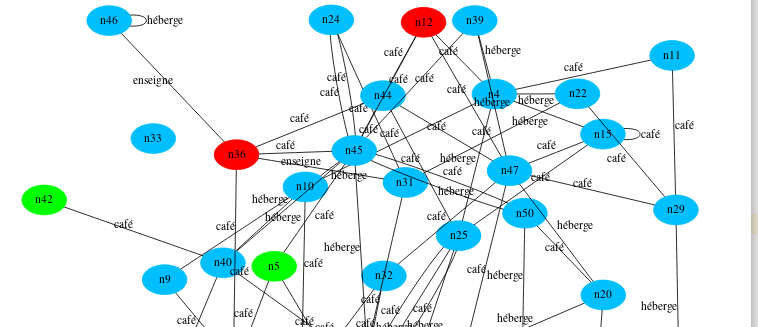
\includegraphics[width=13cm]{graph.png}
\caption{Exemple de sortie graphique (bleu: étudiant, rouge: enseignant, vert: ingénieur)}
\label{graphique}
\end{center}
\end{figure}

\question Remettez au propre le diagramme de classe de l'ensemble de vos classes. On a bien travaillé !

\newpage

\section{Pour aller plus loin...}

\subsection{Généricité}

Vous avez remarqué que dans les classes des relations, par exemple "enseign à", les constructeurs utilisent des "Node". En effet, le constructeur doit avoir la même signature que le constructeur parent. On peut résoudre ce problème en utilisant des génériques.

\quest Copiez votre code dans un autre package. Essayez de modifier vos arêtes pour qu'elles deviennent génériques.

\quest Dans cette version, peut-on mieux gérer plus facilement les contraintes sur les relations entre deux personnes ?

\subsection{Définir le comportement d'affichage comme une interface}

\quest Dans ce TP, nous avons un peu mélangé le fait d'être un graphe, un noeud, une arête et le fait de devoir s'afficher: certaines méthodes du graphe ou de l'arête concernent des aspects d'affichage. Pour être plus propre, on pourrait définir les comportements d'affichage dans une interface. Puis, on pourrait dire que les graphes implémente cette interface. Si l'on veut qu'un graphe ne soit pas obligatoirement afficheable, on peut le faire à un niveau inférieur i.e. un GrapheDePersonne qui implémente cette interface. Cela va de même pour le noeud ou l'arrête: les personnes et les relations impémenteraient l'interface qui définit le comportement d'affichage. Vous pouvez tenter de réaliser cette modification.

\appendix

\section*{Annexes}

\section{Test de getEdges()}
\label{getEdges}

\lstinputlisting[style=java]{../codes/Graphes/src/GraphTest.java}

\section{Test de connexe()}
\label{connexe}

\lstinputlisting[style=java]{../codes/Graphes/src/ConnexeTest.java}

\section{Test des relations}
\label{relation}

\lstinputlisting[style=java]{../codes/Graphes/src/RelationTest.java}



\end{document}
